\documentclass[11pt]{article}

\usepackage{amsmath}
\usepackage{amssymb}
\usepackage{amsthm}
\usepackage{hyperref}
\usepackage{ulem}
\usepackage{enumitem}
\usepackage[left=0.75in, right=0.75in, bottom=0.75in]{geometry}
\usepackage{graphicx}
\usepackage{float}
\usepackage{fancyhdr}
\pagestyle{fancy}
\fancyhf{}
\lhead{190100044 \& 190100055}
\rhead{CS 215: Assignment 1}
\renewcommand{\footrulewidth}{1.0pt}
\cfoot{Page \thepage}

\title{Assignment 1: CS 215}
\author{190100044 \& 190100055}
\date{31st August 2020}

\begin{document}

\maketitle
\tableofcontents
\thispagestyle{empty}

\newpage \setcounter{page}{1}
\section{Question 1}
\begin{enumerate}[label=(\alph*)]
    \item The probability that the first person picks up his/her own book is $\frac{1}{n}$, for the second person, there are $n-1$ books remaining, thus the probability for him/her is $\frac{1}{n-1}$, similarly, the $i^{th}$ person has $ (n-i+1) $ choices, out of which $1$ is correct, thus $P(E_i)$, the probability that the $i^{th}$ person picks up his/her own book is given by: $\frac{1}{n-i+1}$.\\
    Thus, the probability that each person picks up his/her own book ($ \cap_{i=1}^{n} P(E_i) $) is given by:
    $$ \prod_{i=1}^n \Big( \frac{1}{n-i+1} \Big) = \frac{1}{n!}$$
    
    \item Similar to the previous case, we have, the probability that the first $ m < n $ persons who picked up a book receive their own book back again ($ \cap_{i=1}^{m} P(E_i) $),
    $$ \prod_{i=1}^m \Big( \frac{1}{n-i+1} \Big) = \frac{(n-m)!}{n!} $$
    
    \item The first person to pick a book now has $m$ correct choices out of $n$, similarly, the second person has $m-1$ correct choices out of $n-1$ books. Thus, the $i^{th}$ person ($ i \le m $) has $ (m-i+1) $ correct choices, out of $(n-i+1)$ choices. Thus $P(E_i)$, the probability that the $i^{th}$ person ($i < m$) gets back a book belonging to \textbf{one} of the last $m$ persons is equal to: $\frac{m-i+1}{n-i+1}$.\\
    Thus, the probability that each person among the first $m$ persons to pick up the book gets back a book belonging to one of the last $m$ persons to pick up the books is: ($ \cap_{i=1}^{m} P(E_i) $)
    $$ \prod_{i=1}^m \Big( \frac{m-i+1}{n-i+1} \Big) = \frac{m!(n-m)!}{n!} $$
    
    \item The first $m$ persons can pick up any book and each book needs to be clean. Thus $P(E_i)$, the probability that the $i^{th}$ person picks up a book which is clean, is equal to $(1-p)$.\\
    Thus, the probability that each person among the first $m$ persons picks up a clean book is: ($ \cap_{i=1}^{m} P(E_i) $)
    $$ (1-p)^m $$
    
    \item Exactly $m$ persons\footnote{Note that these $m$ persons \textbf{may not} be the first $m$ persons} need to pick up a clean book.\\
    Thus, the ways to choose $m$ persons out of $n$ is ${n\choose m}$, all these chosen people must have chosen a clean book (probability: ($1-p$)), while all the ($ n-m $) remaining people must choose an unclean book (probability: $p$), since it is mentioned \textbf{\textit{exactly}} $m$ persons must choose a clean book.\\
    Thus this probability is given by:
    $$ {n\choose m} (1-p)^m (p)^{n-m} $$
    
\end{enumerate}

\newpage
\section{Question 2}
By the definition of the variance\footnote{Note: Here $\sigma$ is defined to be the \textbf{positive} square root of the variance}, $\sigma^2$, we have:
$$ \sigma^2 = \frac{\sum_{i=1}^n (x_i - \mu)^2}{n-1} $$
\begin{equation}
    \label{var}
    (n-1)\sigma^2 = \sum_{i=1}^n (x_i - \mu)^2
\end{equation}
Since $(x_i - \mu)^2 \ge 0 \  \forall \ i$, we have ((for all $i$)):
$$ \sum_{i=1}^n (x_i - \mu)^2 \ge (x_i - \mu)^2  $$
Thus, by (\ref{var}) we get (for all $i$):
$$ (n-1)\sigma^2 \ge (x_i - \mu)^2 $$
Taking the square root on both sides,
$$ \sigma\sqrt{n-1} \ge |x_i - \mu| \Rightarrow |x_i - \mu| \le \sigma\sqrt{n-1} \hfill $$
\hfill \qedsymbol \\
\noindent
The (Two-sided) Chebyshev's inequality states that:
$$ |S_k| = \{ x_i : \  |x_i - \mu| \ge k\sigma \} $$
\begin{equation}
    \frac{|S_k|}{n} < \frac{1}{k^2}
\end{equation}
Consider $k = \sqrt{n-1}$ in the above equation,\\
$$ |S_{n-1}| = \{ x_i : \  |x_i - \mu| \ge \sigma\sqrt{n-1} \} $$
$$ \frac{|S_{n-1}|}{n} < \frac{1}{n-1} $$

``TODO: How does this inequality compare with Chebyshev's inequality as n increases?"

\newpage
\section{Question 3}

\newpage
\section{Question 4}
Let $A$ be the event that the rickshaw is red.\\
Thus, as a given rickshaw must be either red or blue, $A^c$ is the event that the rickshaw is blue.\\
Let $B$ be the event that the rickshaw is observed as red by the person under the given conditions.\\
We have been given the following:
$$ 
    P(A) = \frac{1}{100} \Rightarrow P(A^c) = \frac{99}{100}
$$
$$
    P(B|A) = 0.99 \ \  P(B|A^c) = 0.02
$$
We need to find $P(A|B)$. \\
\\
We shall first find $P(B)$,
$$
\begin{aligned}
    P(B) &= P(B|A)P(A) + P(B|A^c)P(A^c)\\
    &= 0.99\times0.01 + 0.02\times0.99\\
    &= 0.0297
\end{aligned}
$$
\\
Now, by Bayes Theorem,
$$
\begin{aligned}
    P(A|B) &= \frac{P(B|A)P(A)}{P(B)}\\
    &= \frac{0.99\times0.01}{0.0297}\\
    &= \frac{1}{3} = 0.33 = \mathbf{33\%}
\end{aligned}
$$
Thus, the defence lawyer can argue that there was only a $33\%$ chance that the rickshaw observed by the person XYZ was indeed red.

\newpage
\section{Question 5}

\newpage
\section{Question 6}
\begin{figure}[H]
    \centering
        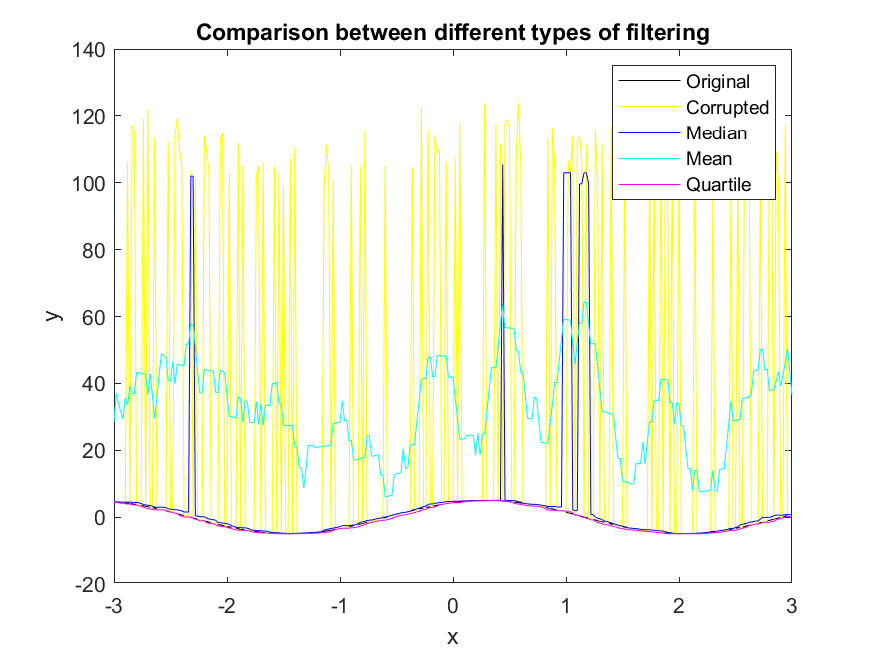
\includegraphics[scale=0.9]{q6.1.png}
\end{figure}
\begin{figure}[H]
    \centering
        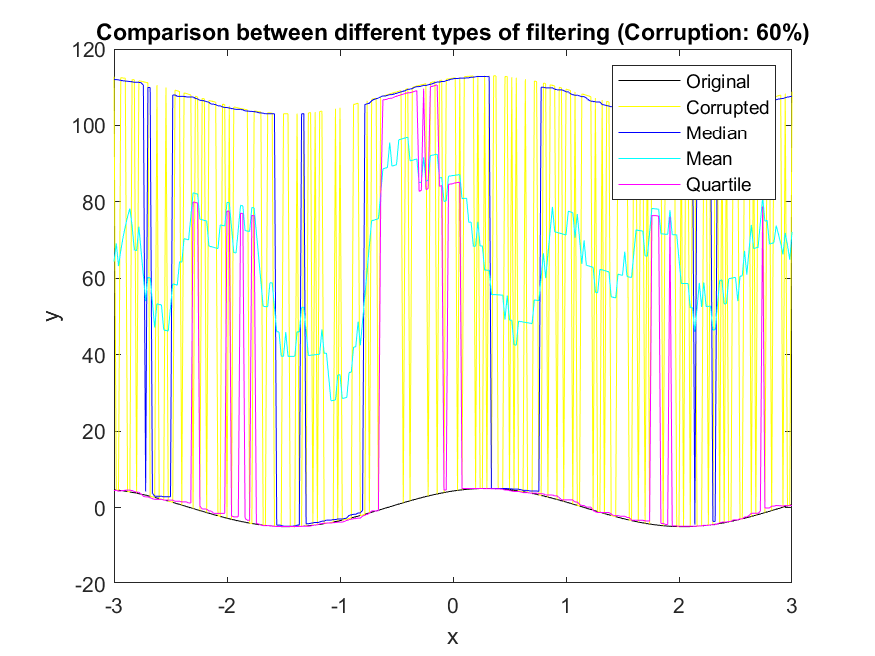
\includegraphics[scale=0.9]{q6.2.png}
\end{figure}  
\begin{center}
    \begin{tabular}{ |c|c|c| } 
        \hline
        \textbf{Results} & \textbf{Mean Square Error (30\% Corruption)} & \textbf{Mean Square Error (60\% Corruption)}  \\ 
        \hline
        Corrputed & 266.09 & 588.35\\
        \hline
        Median & 26.52 & 372.31\\
        \hline
        Mean & 90.15 & 737.09\\
        \hline
        Quartile & 0.01 & 117.38\\
        \hline
    \end{tabular}
\end{center}
\noindent
\textbf{Quartile} method produced the best relative mean squared error.
\subsection*{Explanation:}





\newpage
\section{Question 7}

\end{document}